\section{Installation}
\label{sec:fdsp-coord-install}
%						15 pages

%%%%%%%%%%%%%%%%%%%%%%%%%%%%%%%%
\subsection{Organization}
\label{sec:fdsp-coord-org}

Technical Coordination (TC) is responsible for detector
integration and installation support. On the surface TC is responsible for coordinating with
the LBNF logistics effort and acting as the interface to LBNF
logistics for planning transport of all detector equipment underground. TC
will receive equipment from the consortia and plan the transport to the
Ross shaft with the LBNF logistics coordinator. This will require that
TC receive equipment, will support the consortia in repackaging (and
test the equipment if needed) and preparing the equipment for
transport underground. Given possible delays in shipping a
one month material buffer is foreseen near the SURF site. This effort
will need warehouse space with associated inventory system, storage
facilities, material transport equipment and access to trucking. As a
substantial facility is required near the SURF site this
infrastructure could also be used and a location for the detector
integration facility where detector components from different
consortia are assembled and tested before going underground. The
location of the integration facility will be decided prior to the TDR
and an engineering design of the needed infrastructure will be
available.

TC is responsible for coordinating and supporting the installation of
the detector. The consortia are responsible for the installation of
their equipment, but in order to do this, essential infrastructure
will need to be available. The installation scope includes the
infrastructure needed to install the detector such as the cleanroom,
special cranes, access equipment, basic tools, etc. TC will provide
trained personnel to operate the installation infrastructure. The
consortia will provide the detector elements and custom tooling and
fixtures as required. In the case of the single-phase detector TC will
also provide the detector support system 
needed to bring equipment into the cryostat. TC will supply general
detector specific infrastructure like racks, cable trays, power, and
if needed additional optical fibers in the shafts.

Installation scope is divided into surface and underground
activity. Both the surface and underground scope will be organized
similarly to consortia, with responsibility shared by a scientific
lead and a technical lead. Though organized similarly to the consortia
the surface and underground installation organizations report directly
to the Technical Coordination. These efforts will be referred to as
the Surface team and the Underground installation team (UIT). Clearly
the surface team which delivers equipment to the Ross Shaft and the
UIT which receives the equipment underground need to be in close
communication. The organization of the full installation scope into
work packages that are associated with the different phase of the
project and the lower level WBS divisions are shown in
Figure~\ref{WP_def}.
\begin{figure}[htb]
  \begin{center}
    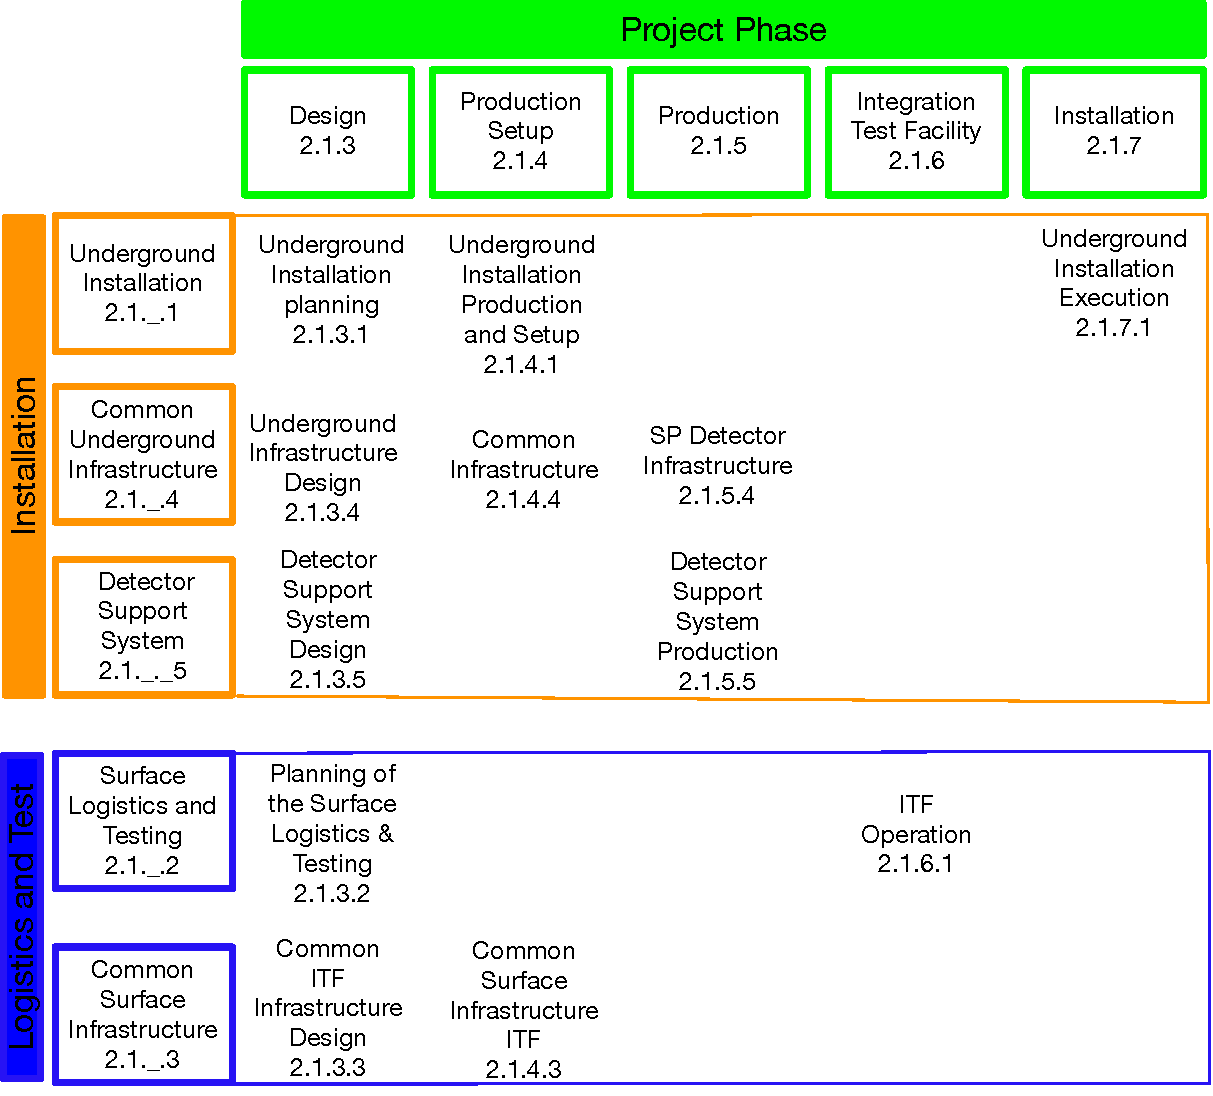
\includegraphics[width=0.8\textwidth]{far-detector-single-phase/figures/OrgChart-v3.pdf}
    \caption{Organization of installation and Surface Logistics and
      Testing. The columns in the matrix represent the project phase
      and the rows the major divisions in scope. Work packages define
      the deliverables for each phase according to the major division
      in scope. }
    \label{WP_def}
  \end{center}
\end{figure}
The main deliverables of the installation team are the
detector installation itself including coordinating the installation
planning, constructing the installation infrastructure and supporting
the installation process. In addition the Underground installation
also provides common detector infrastructure and the DSS. The surface
team or the logistics and test team are responsible for planning
DUNE work on the surface, providing the infrastructure needed
for the logistics, testing and integration and operation of the
facility itself. The DUNE production phases are divided into
production setup and production. Scope that represents a one time
investment is included in production setup while equipment and
infrastructure that scales with the number of detectors is included in
production. With this definition several of the possible work packages
are empty. For example once the surface logistics facility is setup it
will be used for all 4 detectors so its scope is completely under
production setup.

The costs for the installation related scope will in general be
estimated at the work package level for the production and execution
phases of the project. During the design phase a single cost estimate
for installation will be generated. Table~\ref{Instal-Cost} shows the
initial estimates where the work packages are rolled up to the level
of major deliverables.
\begin{table*}[h]
  \begin{center}
    \begin{tabular}{|c|l|c|c|}      \hline
      WBS&Deliverable&Core Cost (k\$)&Labor (FTE)\\      \hline \hline
      2.1.3&Design&&\\      \hline
      2.1.\_.1&Underground installation&&\\      \hline
      2.1.\_.4&Common Underground  Infrastructure&&\\      \hline
      2.1.\_.5& Detector Support System&&\\      \hline
      2.1.\_.2&Surface Logistics and Testing&&\\ \hline
      2.1.\_.3&Common Surface Infrastructure&&\\ \hline
    \end{tabular}
  \end{center}
  \caption{Summary of the installation costs. }
  \label{Instal-Cost}
\end{table*}


%%%%%%%%%%%%%%%%%%%%%%%%%%%%%%%%
\subsection{Surface Logistics \& Testing}
\label{sec:fdsp-coord-integ-test}

The logistics for integrating and installing the DUNE Far Detectors
and their associated infrastructure face a number of
challenges. Possible difficulties include the size and complexity of
the detector itself, the number of sites around the world that will be
fabricating detector and infrastructure components, the necessity for
protecting components from dust, vibration and shock during their
journey to the deep underground laboratory and the lack of space on
the surface near the Sanford Lab Ross Shaft. One mitigation
of these risks is the establishment of a DUNE
Integration and Test Facility (ITF) somewhere in the vicinity of
Sanford Lab. Such a facility and its associated staff would contribute
to DUNE in the following areas.
\begin{itemize}
  \item {\bf Transport Buffer:} Storage capacity for one month
    material in the vicinity of Sanford Lab. Handle packaging
    materials returned from underground laboratory.
  \item {\bf Re-packaging} Facilitate possible re-packaging of
    components before transport underground.
  \item {\bf Component Fabrication:} Possibly provide a capability for
    fabrication of components near Sanford Lab. Undergraduate science
    and engineering students from the South Dakota School of Mines and
    Technology (SDSM\&T) may contribute low cost effort to these
    fabrication activities.
  \item {\bf Component Integration:} Some integration activities may
    be best accomplished in proximity to Sanford Lab. A possible
    example is connecting photodetectors and cold electronics to APAs.
  \item {\bf Inspection, Testing and Repair:} Consortia will define
    their testing requirements including procedures and
    criteria. Consortia will also specify procedures in cases of test
    failure, for example, repair, return to source or discard.
  \item {\bf Visitor Support:} Consortia will likely send staff to the
    ITF for the integration, testing and installation of the consortia
    detector components. The ITF will provide temporary space,
    computer access, assistance personnel and other infrastructure
    support for DUNE visitors.
%\item {\bf Outreach:} The ITF may be well located to support a public outreach program. The DUNE Experiment is likely to generate considerable public interest and addressing those interests is important to long-term public support for DUNE specifically and particle physics generally.
\end{itemize}

\subsubsection{Scope}
The scope of the ITF includes several possibly related but mostly
independent tasks. They are:
\begin{itemize}
\item{\bf Cryostat:} The scope of this item is the four cryostats
  planned for installation at the 4850 level of Sanford Lab. Cryostat
  components include the warm steel structure, the stainless steel membrane and
  the insulation. The logistics for the cryostat components will be
  managed by the cryostat installation contractor and LBNF logistics
  coordinator.  Most likely this function will be met with a
  commercial warehousing vendor, who will supply suitable space,
  loading and unloading facilities and a commercial inventory
  management and control system. The vendor will provide all required
  personnel effort as part of its contracted responsibilities.
\item{\bf Cryogenics Systems:} The cryogenics systems are also an LBNF
  responsibility and cryogenics system logistics will likely be
  managed by LBNF similarly to the logistics for the cryostat
  components.
\item{\bf Cryostat Support Structure:} This structure is an LBNF
  responsibility and will likely be addressed similarly to the
  Cryostats and the Cryogenic Systems.
\item{\bf DUNE Detectors:} The DUNE Detectors are the responsibility
  of the Collaboration as implemented by the Consortia. The role of
  the ITF will vary for the several Consortia and a description of
  these various roles is a major topic of this document.
\end{itemize}

\subsubsection{Location }
A reasonable criterion for the location of the ITF is within about an
hour drive from Sanford Lab. That criterion yields the following
possibilities.
\begin{center}
\begin{tabular}{ |c|c| } \hline
{\bf Location} & {\bf 2016 Population}  \\ \hline 
Deadwood & 1,264  \\ 
Lead & 3,010  \\
Rapid City & 74,048  \\
Spearfish & 11,531  \\
Sturgis & 6,832  \\ \hline
\end{tabular}
\end{center}
Since infrastructure is correlated with population, Rapid City would seem the most likely
choice for location with Spearfish as a second possibility. In addition to overall infrastructure,
particular assets of Rapid City include proximity to SDSM\&T and a business community that is
possibly interested in incorporating a DUNE ITF into an overall regional development
program.
%Black Hills State University is located in Spearfish, but that institution is less technology oriented than SDSM\&T.

\subsubsection{Management:}
The management of the ITF should likely be provided by one or more
DUNE Collaborating Institutions. A possible choice is SDSM\&T because
of its physical proximity, its understanding of the local
infrastructure and relationships and its ability to provide some
specialized effort and specialized facilities that might benefit
the ITF.  Some preliminary discussions with SDSM\&T management
have already occurred. These discussions should be ongoing as the
parameters for the ITF become more definite.
\begin{center}
\begin{tabular}{|l|c|c|c|c|c|c| } 
\hline
{\bf Consortium} & {\bf Transport} &{\bf Re-Packaging}&{\bf Component}
&{\bf Component}&{\bf Inspection,}&{\bf Visitor} \\
 & {\bf Buffer} &{\bf }&{\bf Fabrication}
&{\bf Integration}&{\bf Testing}&{\bf Support} \\\hline 
High Voltage & Yes & Yes & No & Yes? & Yes & Yes \\ \hline
APA & Yes & Yes & Yes & Yes & Yes & Yes \\ \hline
DAQ & Yes & Yes & Yes & Yes & Yes & Yes \\ \hline
CE-SP & Yes & Yes & No & No & Yes & Yes \\ \hline
CE-DP & Yes & No & No & No & Yes & Yes \\ \hline
PD-SP & & & & & &  \\ \hline
PD-DP & Yes & Yes & Yes & No & Yes & Yes \\ \hline
Slow Control & & & & & &  \\ \hline
CRP & & & & & &  \\   \hline
\end{tabular}
\end{center}
\begin{center}
\begin{tabular}{|l|c|c|} \hline
{\bf Consortium} & {\bf Leaders} &{\bf Respondents} \\ \hline
High Voltage & Francesco Pietropaolo, Bo Yu & Bo Yu \\ \hline
APA & Stefan Soldner-Rembold, Alberto Marchionni & Peter Sutcliffe \\ \hline
DAQ & Georgia Karagiorgi, Dave Newbold & Alec Habig \\ \hline
CE-SP & & \\ \hline
CE-DP & D. Autiero, T. Hasegawa &  D.Autiero  \\ \hline
PD-SP & & \\ \hline
PD-DP & Ines Gil Botella, Dominique Duchesneau & Burak Bilki \\ \hline
Slow Control & &   \\ \hline
CRP & &  \\   \hline
\end{tabular}
\end{center}

\subsubsection{Inventory System:}
Effective inventory management will be essential for all aspects of
DUNE detector development, construction, installation, and operation.
While its relevance and importance go beyond the Integration and Test
Facility, the ITF is the location at which LBNF, DUNE project
management, consortia scientific personnel, and SURF operations will
interface.  We therefore will develop standards and protocols for
inventory management as part of the ITF planning.  A critical
requirement for the project is that the inventory management system
for procurement, construction and installation must be compatible with
future QA, calibration and detector performance database systems.
Experience with past large detector projects, notably NOvA, has
demonstrated that the capability to track component-specific
information is extremely valuable throughout installation, testing,
commissioning, and routine operation.  Compatibility between separate
inventory management and physics information systems will be
maintained for effective operation and analysis of DUNE.

DUNE will rely on a commercial vendor for warehouse and logistics
services in Rapid City or another location nearby to SURF.  Warehouse
vendors have a variety of inventory software packages and standards,
and final specification of the DUNE/LBNF system cannot happen until
the project warehouse vendor is selected.  Discussions are being
coordinated closely with LBNF and initial visits and meetings with
warehouse vendors and software suppliers have occurred.  DUNE
scientific personnel will continue to evaluate candidate systems and
assure interoperability with a future physics database
information systems.

Because of the widely distributed nature of the DUNE development and
construction project and the required compatibility with a commercial
warehouse management system, we plan to develop core inventory
management capabilities based on a service-oriented architecture.  URL
connections will be used to pass data (JSON format) to RESTful APIs,
which have task-specific code written in Python that communicates with
standard PostgresSQL database that will be developed for DUNE by
Fermilab.  Specialized code at remote sites would also be in Python.

Implementation within a commercial cloud-based computing environment,
well suited to the international DUNE project, is also under
consideration.  A recent visit to Rapid City revealed that Dakota
Warehouse
(\href{https://dakotawarehouse.com}{https://dakotawarehouse.com}), a
leading candidate for providing LBNF/DUNE warehouse services for
detector components, including cryostat and cryogenic systems, uses a
cloud-based commercial software package, 3PL Central
(\href{https://3plcentral.com}{https://3plcentral.com}), in which
orders of shipments and stock status are entered and queried through
an internet browser interface.  We will consider the feasibility of
this or a similar platform for LBNF and DUNE.

%%%%%%%%%%%%%%%%%%%%%%%%%%%%%%%%
\subsection{Underground Detector Installation}
\label{sec:fdsp-coord-undergd}

\fixme{This section is very detailed. We need to be more concise.}
For the DUNE detectors to be installed in safe and efficient manner
the effort of the individual consortia need to be coordinated such
that the installation is planned as a coherent process. The interfaces
between the individual components needs to be understood and the
spaces required for the installation process planned and
documented. The installation planning needs to take into account the
plans and scope of the LBNF effort and the individual plans of the
nine consortia. By working with the LBNF team and the members of the
consortia responsible for building and installing their components, a
joint installation plan and schedule taking into account the all the
activities and needs of all the stakeholders can be developed. Though
the organization of the installation effort is still evolving it is
assumed in this document that the underground installation team (UIT) will be organized
similarly to the consortia. For the installation team the equivalent
of the scientific lead is the installation coordinator (IC) and and
the technical lead the installation technical lead (ITL). The UIT
leadership will be appointed prior to the TDR approval along with the
UIT staffing plan and material basis of estimates (BOEs).

One of the primary early responsibilities of the Underground
installation Team (UIT) after its formation will be to review and
maintain the DUNE installation plan and the installation schedule. The
DUNE installation plan will describe the installation process in
sufficient detail to demonstrate how all the individual consortium
installation plans mesh and it will give the overview of the
installation process. The UIT will be responsible for reviewing and
approving the consortia installation plans. Approved installation
plans, engineering design notes, signed final drawings, Safety
documentation and procedures are all prerequisites for the Production
Readiness Reviews (PRR). Approved procedures, safety approval, and
proper training are all required before the UIT will perform work.
  
During the installation phase the installation leadership will
coordinate the DUNE installation effort and adapt the schedule as
needed. The installation coordinator with management will also resolve
issues when problems occur. Common installation infrastructure will
also be part of the installation scope. This includes: the underground
class 100k clean room, cranes and hoists (if they are not delivered by
LBNF), scissor lifts, areal lifts, and the common work platforms
outside the cryostat. The UIT will have responsibility for operating
this equipment and assisting the consortia with activities related to
rigging, material transport, and logistics. {\bf Each consortium is
  responsible for the installation of their own equipment so the
  responsibility of the installation group is limited but the material
  handling scope is substantial.} To support the installation process
an installation foreman will lead a trained crew with the main
responsibility of transporting the equipment to the necessary location
and operating the cranes, hoists, and other common equipment needed
for the installation. It is expected that the installation crew will
work with the teams from the various consortia but will mainly act in
a supporting function. The UIT foreman will be responsible for
supervising the UIT crew, but the ultimate responsibility for all
detector components will remain with the consortia even while the
underground team is rigging or transporting these components.  This
will be critical in case parts are damaged during transport or
installation, as the consortia need to judge the necessary
actions. For this reason, a representative or point-of-contact (POC)
from the consortia must be present when any work is performed on their
equipment. The consortium is responsible for certifying that each
installation step is properly performed.

The UIT acts as the primary point of contact with LBNF/SURF from the
time the components reach the headframe until the equipment reaches
the experimental cavern (if something goes wrong SURF calls the UIT
leader who then contacts the responsible party). The consortia are
responsible for delivering to the UIT all approved procedures and
specialized tooling required for transport. The UIT leader acts as a
point of contact if the LBNF/SURF team has questions or difficulties
with the underground transport.  The UIT receives the materials from
LBNF/SURF at the entrance to the DUNE excavations. The UIT then
delivers the equipment to the required underground location.

In an effort to get an early estimate of the equipment required, the
spaces needed and the time required for the installation the
installation Planning Team (IPT) has begun the process of generating a
preliminary installation procedure and is working with the consortia to
come to a baseline installation plan. The UIT will take ownership of
the plan once it forms.
\fixme{images are too small}
\begin{figure}[htbp]
\begin{center}
\begin{minipage}[c]{0.49\textwidth}
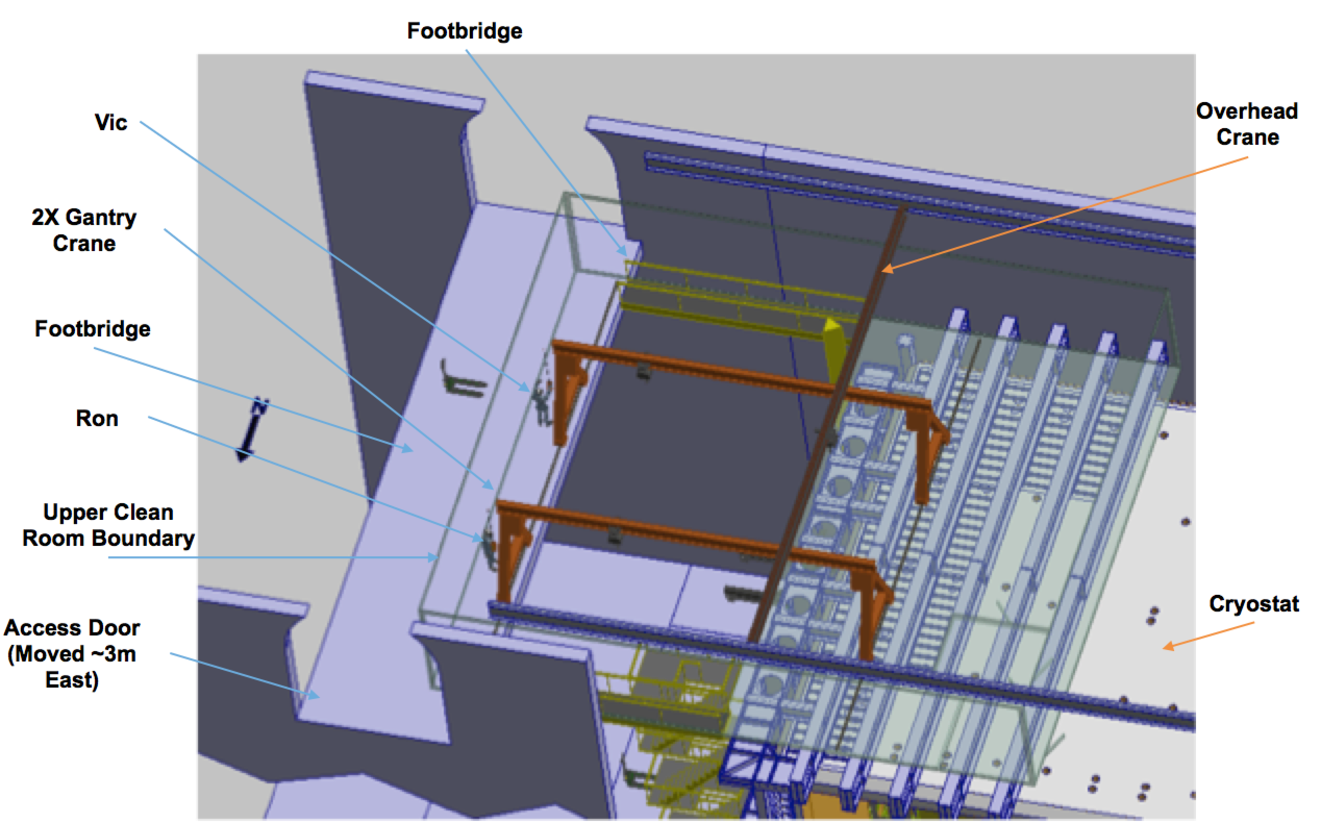
\includegraphics[width=\textwidth]{far-detector-single-phase/figures/Install-ISO-Top.pdf}
\end{minipage}
\begin{minipage}[c]{0.49\textwidth}
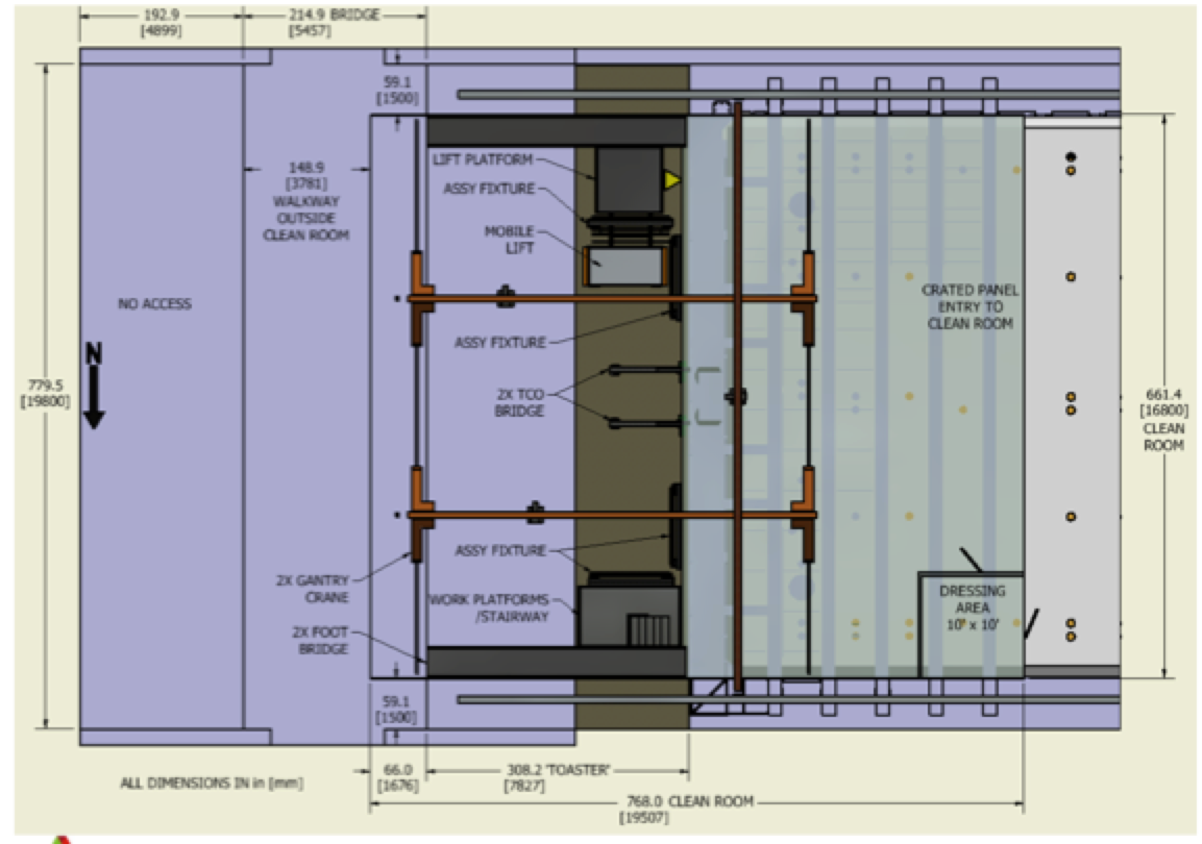
\includegraphics[width=\textwidth]{far-detector-single-phase/figures/Install-TopView.pdf}
\end{minipage}
%
\vspace{5mm}
\hrule
\vspace{5mm}
%
\begin{minipage}[c]{0.32\textwidth}
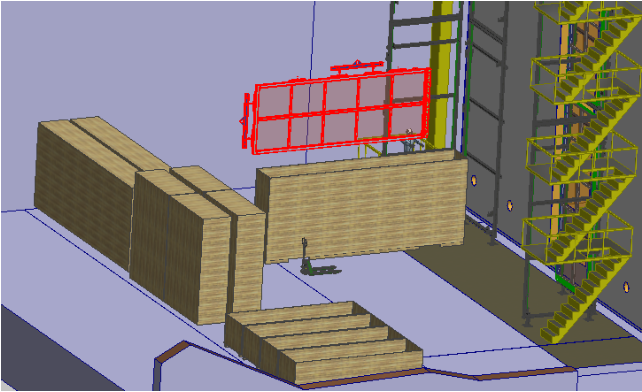
\includegraphics[width=\textwidth]{far-detector-single-phase/figures/APA-1.pdf}
\end{minipage}
\begin{minipage}[c]{0.32\textwidth}
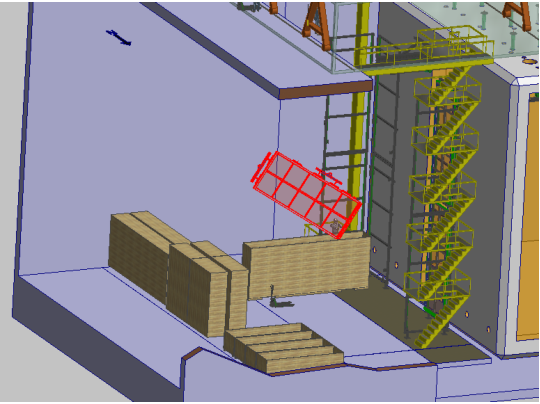
\includegraphics[width=\textwidth]{far-detector-single-phase/figures/APA-2.pdf}
\end{minipage}
\begin{minipage}[c]{0.32\textwidth}
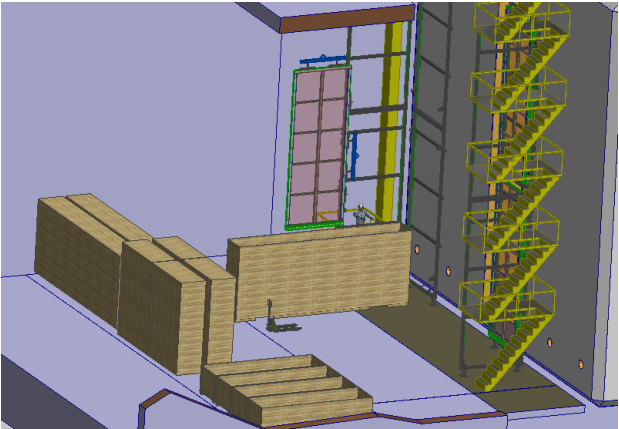
\includegraphics[width=\textwidth]{far-detector-single-phase/figures/APA-3.pdf}
\end{minipage}
%
\vspace{5mm}
\hrule
\vspace{5mm}
%
\begin{minipage}[c]{0.32\textwidth}
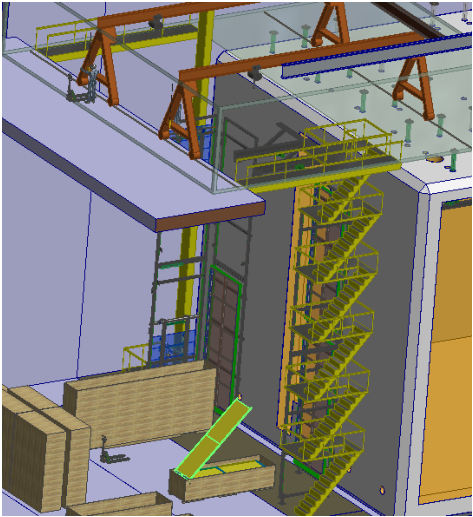
\includegraphics[width=\textwidth]{far-detector-single-phase/figures/CPA-1.pdf}
\end{minipage}
\begin{minipage}[c]{0.32\textwidth}
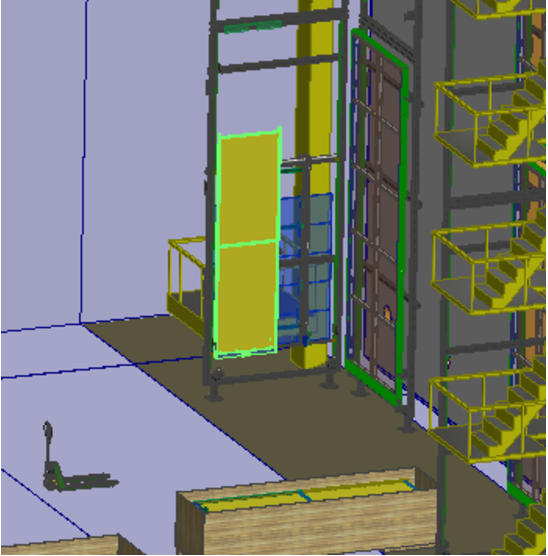
\includegraphics[width=\textwidth]{far-detector-single-phase/figures/CPA-2.pdf}
\end{minipage}
\begin{minipage}[c]{0.32\textwidth}
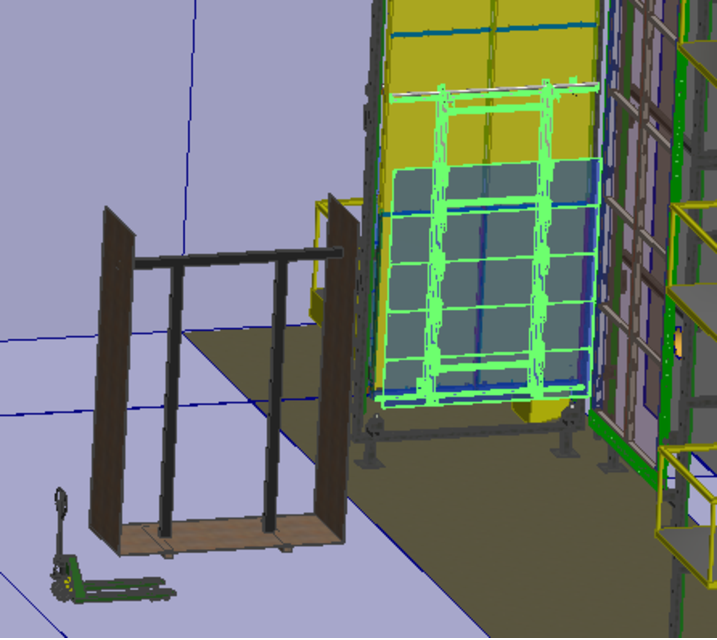
\includegraphics[width=\textwidth]{far-detector-single-phase/figures/CPA-3.pdf}
\end{minipage}

\caption{Installation sequence}
\label{Install-Seq}
\end{center}
\end{figure}



The current installation plan is desscribed. DUNE will take
ownership of the different underground areas at different times. The
surface data room and the underground room in the CUC are available
significantly before the collaboration has access to the cryostats and
the optical fibers between the surface and underground will be in
place even earlier. This will allow a DAQ prototype to be developed
and tested early. The installation of the DAQ hardware can also be
finished before the start of detector installation if desired so the
DAQ will not be on critical path.  When the collaboration receives
access to Cryostat~\#1 the steel work for Cryostat~\#2 will be
finished and the work on installing the membrane will have
started. Excavation will be complete.  The first step in the
installation is to install the cryo-piping and the DSS. As the
cryo-piping will require welding and grinding it is a dirty process
and must be complete before the area can be used as a cleanroom. When
this is complete the cryostat can be cleaned and the false floor
re-installed. The clean infrastructure needed to install the detector
including the cleanroom, work platforms, scaffolding, and the
fixturing to hold the detector elements during assembly and all the
lifts need to be set up. Once the infrastructure is in place and the area
clean the installation of the main elements can start. The general
layout of the installation area showing the necessary space and
equipment is shown in the top panels in Figure~\ref{Install-Seq}.

[Need an image of the detector showing where the endwalls are and where West is. Show 25 rows?]

The SP detector is installed by
first installing the west endwall or endwall~\#1. The the APAs and
CPAs with top/bottom FC panels are installed. The plan is to install 6
APAs and 4 CPAs per week which is enough to complete one of the 25
rows every week. Additional time is built into the schedule to take
into account that the installation will be slower at the beginning and
some re-work may be needed. By building west-to-east complete rows can
be finished and tested before moving to the next row. This reduced the
risk that after final FC deployment and cabling that a fault is found
which require dismantling par of the detector. Some of the steps
needed to install the APA and CPA modules outside the cryostat are
also shown in Figure~\ref{Install-Seq}.  The middle three panels show
how the APA needs to be handled in order to rotate it and mount it to
the assembly frame. After two APA are mounted on top of each other the
cabling for the lower APAs cold electronics and photon detector cables
can be installed. The lower three panels show how the 2m CPA
sub-panels are removed form the transport crates and assembled on
holding frame. Once the CPA module is assembled the Field Cage units
can them be mounted. Finally once the APA and CPA are installed the
endWall~\#2 can be installed. A high level summary of the schedule is
shown in Figure~\ref{Install-Schedule}.
\fixme{light blue in figure does not show up in B\&W}
\begin{figure}[htbp]
\begin{center}
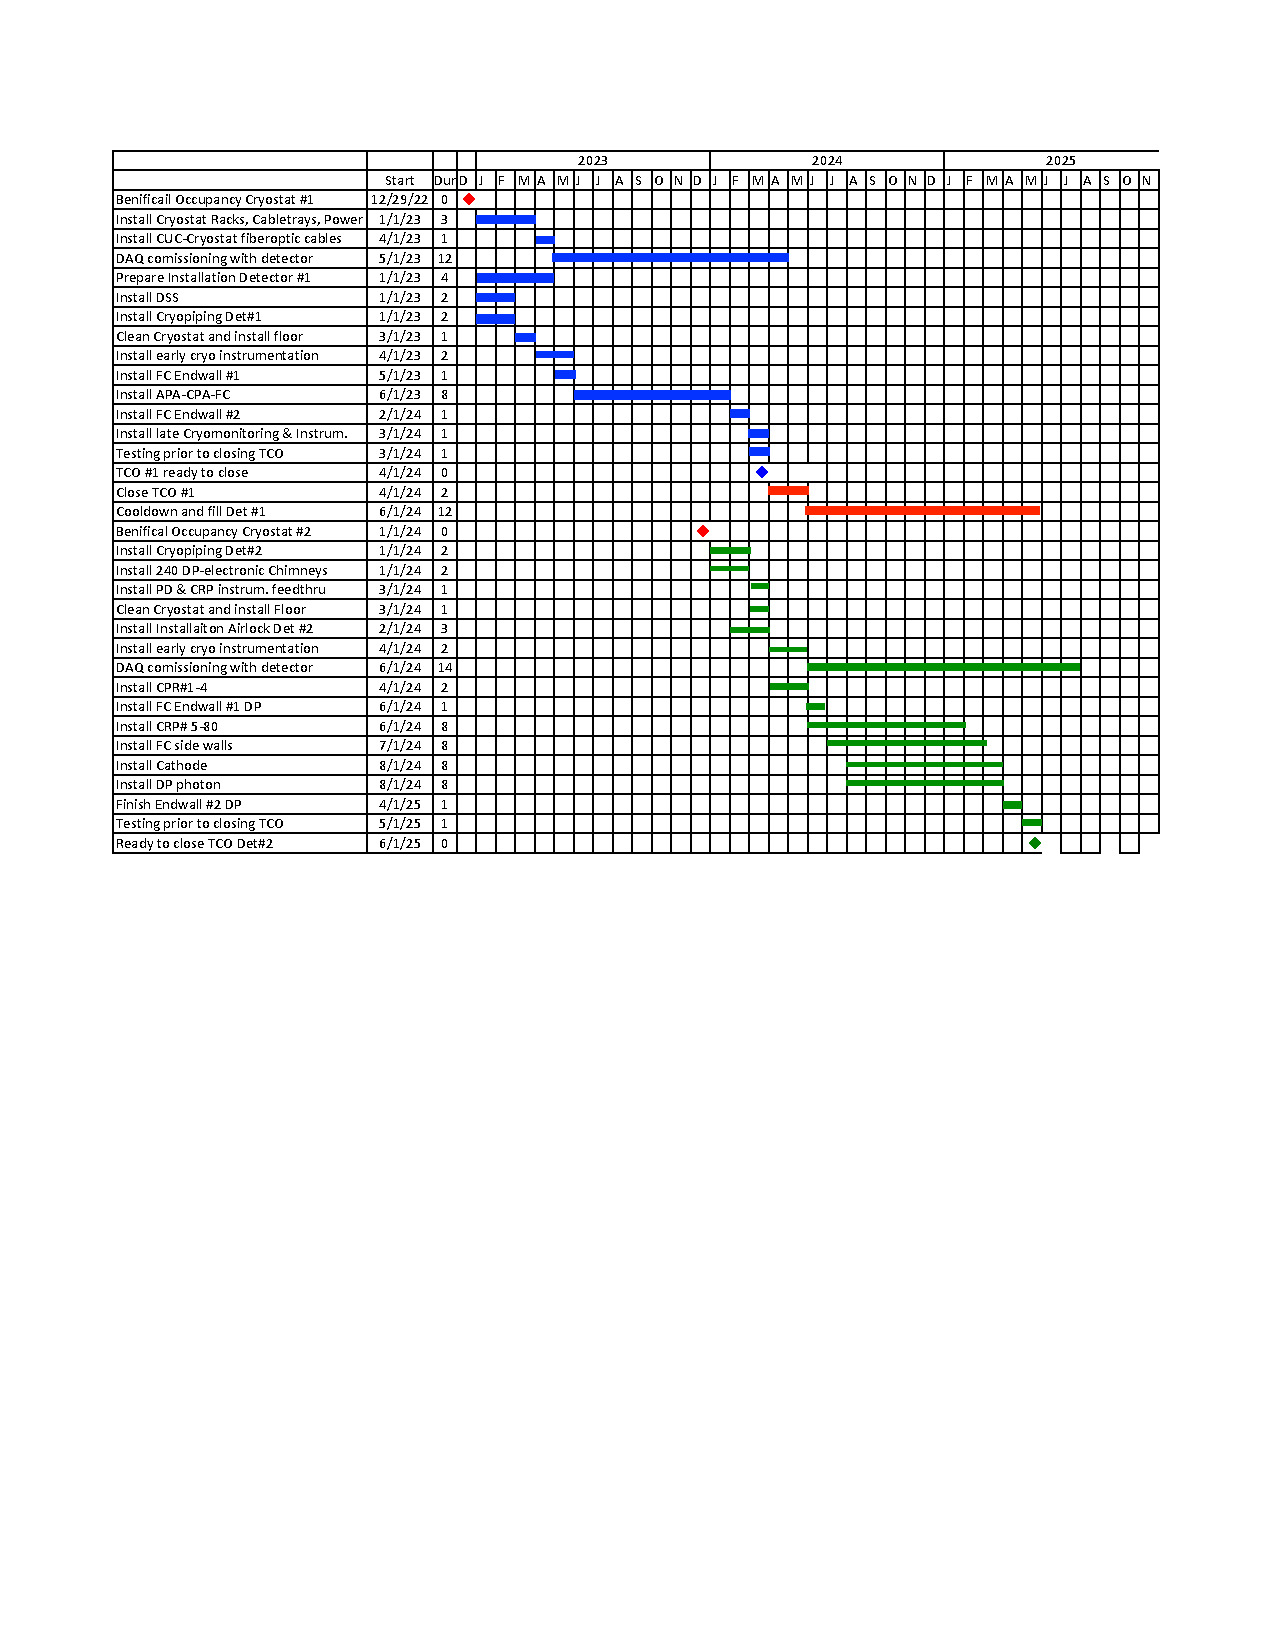
\includegraphics[width=\textwidth]{far-detector-single-phase/figures/TP-Schedule-Feb2018.pdf}
\caption{High level installation schedule}
\label{Install-Schedule}
\end{center}
\end{figure}

[Image of Dual Phase detector?]

Once the first detector is installed work on setting up the second
detector installation can begin. This work includes moving the cranes
and work platforms along with moving the walls of the cleanroom so the
second cryostat is clean. For the purposes of this Technical Proposal
it is assumed that the second detector is a Dual-Phase TPC (DP) with
photon detection. The individual detector elements of the Dual-Phase
TPC are smaller than the SP detector so the installation
infrastructure is simpler. The DP detector will need a cleanroom and
cranes capable of moving the equipment to the cleanroom entrance. Much
of the work for the DP installation will be performed inside the
cryostat. Like the SP detector the first step is the installation of
the cryo-piping followed by cleaning and installation of the false
floor. While the cryo-piping is being installed the DP chimneys for
the electronics along with the DP-PD and CRP instrumentation feedthrus
can be installed. The DP detector requires a much smaller cleanroom
which is installed just outside the TCO. At the start of the TPC
installation the first 4 CRP will be installed which comprises the
first row of CRP. Once the first CRPs are installed and tested then
the first endwall can be installed while the second row of CRP are
installed. In general, after this the assembly sequence will include rows of
CRP and then them rows of FC are installed
followed by the cathode installation and the photon detector
PMTs. Finally at the end the second field cage endwall is installed
and a final testing period for the full detector is foreseen. The DP
installation sequence is shown in magenta in Figure~\ref{Install-Schedule}.

The UIT is responsible for delivering the common infrastructure
the detector will need to operate. This infrastructure is typically
equipment that is used by many groups. This may include: the
electronics racks with power and cooling, cable trays, the cryostat
crossing tubes and flanges, rigging equipment, some tools, the ground
monitoring and isolation transformers, necessary diagnostics equipment
(including oscilloscopes, a network analyzers and leak detector), a
small machine shop, storage with some critical supplies, and some PPE.

Prior to the TDR mutually agreed upon installation plans will need to
be approved. These will set the schedule for the installation and will
determine the planning for staffing and budget. Having good estimates
for the time needed and having enough experience to ensure the
interfaces are understood and the procedures are complete is important
for accurate planning. The experience at ProtoDUNE will be very
important as the ProtoDUNE installation establishes the procedures for
handling all the detector elements and in many cases gives accurate
estimates for the time needed. However in the case of the single-phase
detector many of these procedures need to revised or newly developed
as the DUNE detector will be twice as high as ProtoDUNE so two APAs
need to be assembled together and then a totally different cabling scheme is
needed. Testing the cabling will need to be complete prior to the TDR
as this is needed to ensure the design is viable. The dual-phase will
also need to develop new installation procedures as the DUNE DP
detector will have a significantly different field cage and cathode
plane.

The installation by definition is on the critical path making it vital
that the work be performed efficiently and in a manner that has low
risk. In order to achieve this a prototype of the installation
equipment will be constructed at Ash River and the installation
process tested with dummy detector elements. It is expected that the
setup will be available at the time of the TDR, but any lessons
learned will need to be implemented and tested after this. In the
period just prior to the start of installation the Ash River setup
will be used as a training ground for the UIT.


\subsubsection{Detector Support}

\fixme{This section is very detailed. We need to be more concise.}
The Detector Support System (DSS) provides the main structural support
for the single-phase detector.  The detector elements supported by the
DSS include the field cage endwalls, the APAs, and the CPAs with
top and bottom field cage panels.  The DSS is supported by the cryostat
outer steel structure through a series of feedthrus which cross
through the cryostat insulation and are anchored with flanges on the
cryostat roof. Inside the cryostat a series of stainless steel I-beams
are connected to the feedthrus and used to support the detector. The
DSS defines the location of the detector inside the cryostat and it
also defines how the detector elements move as the detector is
brought to LAr temperature. The design of the DSS encompasses the overall
structural design of the detector as only after the elements are
mounted to the DSS and are connected together do they make a unified
mechanical structure. The requirements of the DSS are as follows:
%\begin{itemize}
%  \item[] {\bf DSS REQUIREMENTS}
%\end{itemize}
\begin{itemize}
 \setlength\itemsep{0 em}
 \small
\item Support the weight, both dry and wet [warm and cold?], of
  the detector (endwall, top/bottom FC, APA, CPA)
\item Accommodate the roof movement [ROOF DEFORMATIONS NEED TO BE DEFINED]
\item Accommodate variation in the feedthrough locations and
  variation in the flange angles due to installation tolerances and
  loading on the warm structure.
\item Accommodate shrinkage of the detector and DSS from ambient
  temperature to LAr temperature.
\item Minimize the gaps that develop between APAs during cool down to
  less than 13~mm. [WHAT IS THE CORRECT VALUE?]  %A proposed  design uses beams that are 6.4m long, which support $\sim$3 APAs.  This design results in no gap developing between the three APAs on  the same beam but a 17~mm gap opening up between adjacent APAs on  separate beams.  There will be a 17~mm gap between every 3$^{rd}$  and 4$^{th}$ APA.
\item Accommodate installation of the detector. 
\item Define the position of the detector components relative to each other. [NEED TO DEFINE THIS TOLERANCE]
\item The CPA to APA centerline distance and tolerance envelope must be maintained at 3574$\pm y$~mm
\item The DSS is electrically connected to the cryostat ground
\item The APA/CPA/FC/endwall are electrically isolated from the DSS
\item The DSS penetrations must be purged with GAr to maintain a positive pressure in order to prevent contaminants from diffusing back into the liquid
\item The instrumentation cabling must not interfere with the DSS.
\item The DSS components must be able to be installed through the TCO
%\item A QA program is required
\item The DSS is to designed to meet AISC-360 and appropriate codes required by SURF
\item The DSS will be designed to meet seismic requirements 1 mile underground at SURF
\item All materials must be compatible for operation in ultrapure LAr
\item The DSS beams will be completely submerged in LAr
\item The DSS will ensure that detector components shall not be less than 400~mm from the membrane flat surface
\item The DSS supports shall not interfere with the cryostat I-beam structures
\item The DSS shall be designed such that it supports the detector so that the lower ground plane is above the cryogenic piping and the top of the DSS beams are submerged in LAr while leaving a 4\% ullage at the top of the cryostat.
\item The DSS shall have infrastructure necessary to move the APA and CPA-FC assemblies from outside the cryostat through the TCO and to the correct position.
\end{itemize}

Figure~\ref{DSS} (left) shows the DSS structure; there are five
rows of supports for the alternating rows of APA-CPA-APA-CPA-APA.  The
DSS is connected to the warm structure at a flange that is mounted on
the outside of the cryostat.  Figure~\ref{DSS} (right) shows the
layout of these structural feedthroughs.  The DSS consists of pairs of
feedthroughs that support 6.4~m-long S8x18.4 stainless steel I-beam
sections. The proposed design of the DSS has 10 I-beam
segments per row for a total of 50 I-beam segments. Each I-beam is
suspended on both ends by rods from feedthroughs that penetrate the
roof.  In the cold condition each beam will shrink which will cause
gaps to form between APAs that are adjacent but supported on separate
beams.  APAs that are supported on the same beam will not have gaps
develop because both the beam and APAs are stainless steel so they
will shrink together.  Each beam is supported by a nearly 2m long rod
that allows the beam support to move as the beam contracts.

\fixme{too much detail}
The feedthrough consists of a flange and $8 ^{''}$ OD structural tube
welded to it that extends through the cryostat insulation.  There is a
nominal 10mm gap between the OD of the tube and the ID of the
clearance tube in the cryostat.  The purpose of the $8 ^{''}$ tube is
to provide lateral support to the I-beams during installation.
Running down the center of the feedthrough is a 1� diameter rod that
is supported at a swivel washer at the flange and then supports the
I-beam at a clevis.  The gas seal is obtained by Conflat Flange and a
bellows that seals around the swivel washer.  The lateral position of
the rod can be adjusted to adjust the height of the DSS I-beams.
\begin{figure}[htbp]
\begin{center}
\begin{minipage}[c]{0.49\textwidth}
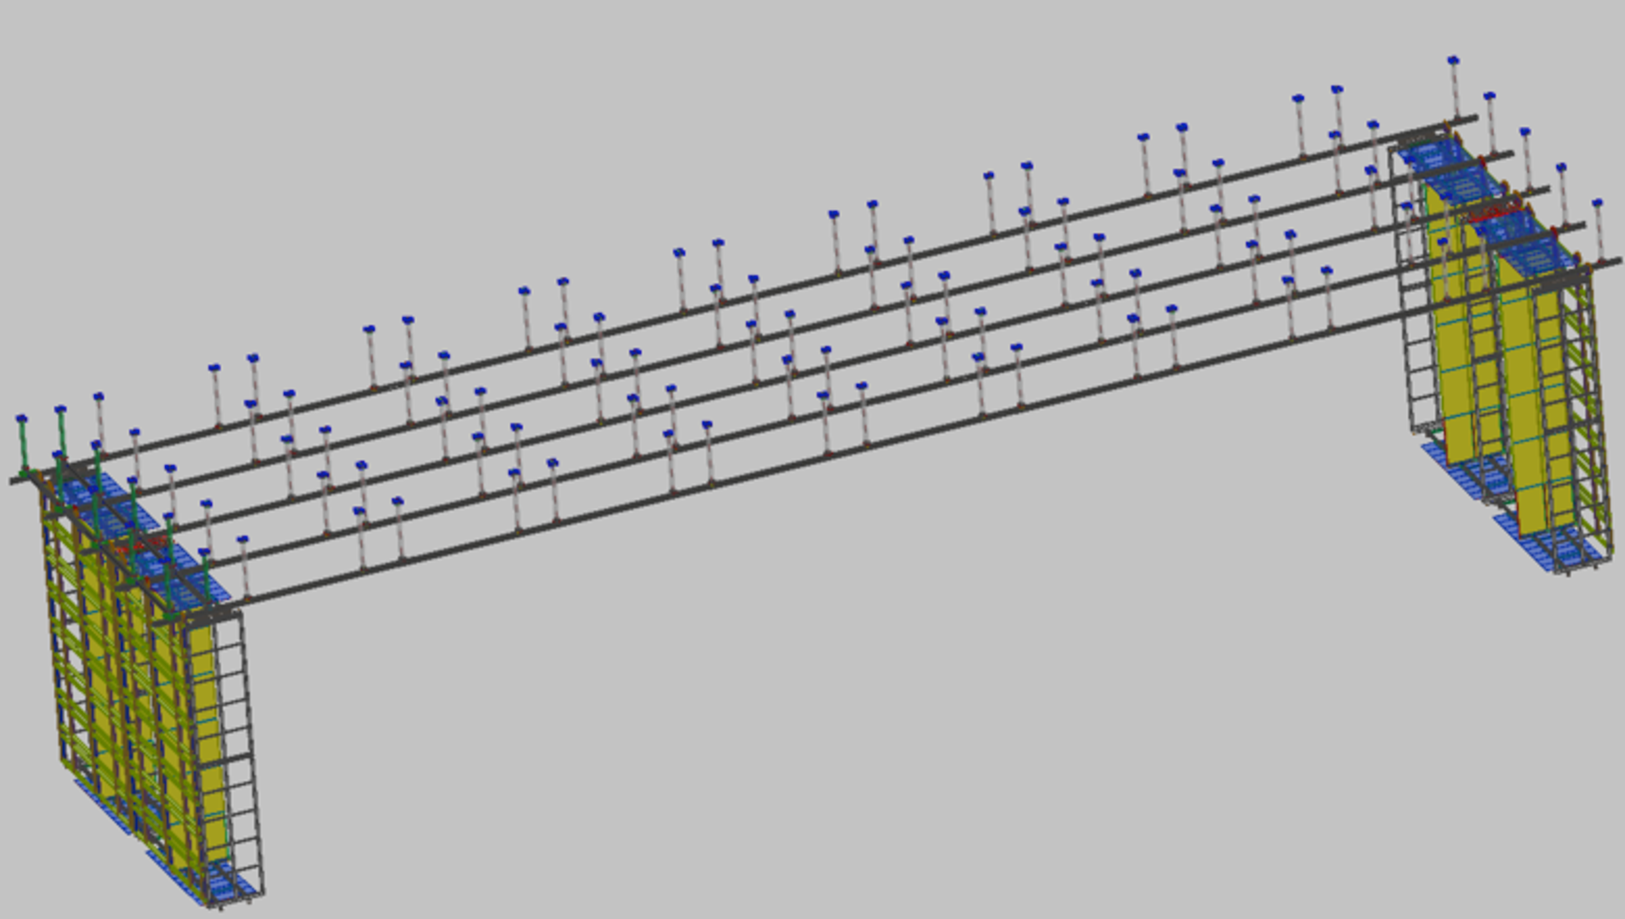
\includegraphics[width=\textwidth]{far-detector-single-phase/figures/DSS-1.pdf}
\end{minipage}
\begin{minipage}[c]{0.49\textwidth}
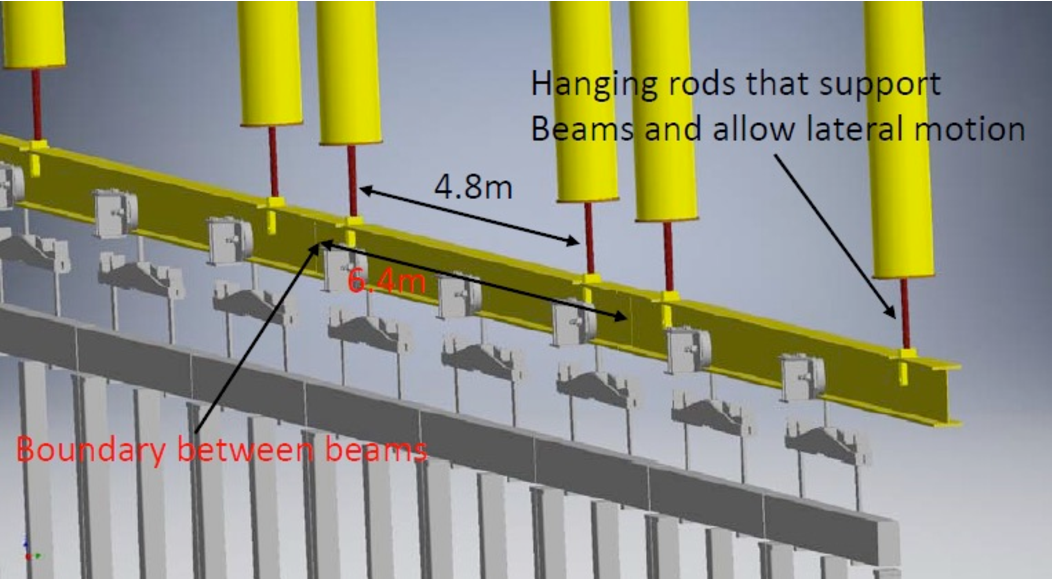
\includegraphics[width=\textwidth]{far-detector-single-phase/figures/DSS-2.pdf}
\end{minipage}
\caption{3-D model of the Detector Support System showing the entire structure on the left along with one row of APA and CPA/FC at each end. The right panel is a zoomed image showing the connections between the vertical supports and the horizontal I-beams.}
\label{DSS}
\end{center}
\end{figure}


Detector components will be installed using a shuttle beam system
illustrated in Figure~\ref{shuttle}.  The last two columns of
feedthroughs (eastern most) will support temporary beams that run
north-south, perpendicular to the main DSS beams.  A shuttle beam
%shown in orange
will have trolleys mounted to it and will transverse
north-south until aligned with the required row of DSS beam.  The last
APA or CPA in a row is supported by the shuttle beam which is bolted
directly to the feedthroughs once it is in place.  As the last CPA or
APA in each row is installed the north-south beams are removed.

There will be a mechanical interlock system that prevents trolleys
from passing the end of the shuttle beam unless it is aligned with a
corresponding DSS beam.  The shuttle beam and each detector will be
moved using a motorized trolley.  A commercially available motorized
trolley will be modified as needed to meet the needs of the
installation.
\begin{figure}[htbp]
\begin{center}
\begin{minipage}[c]{0.49\textwidth}
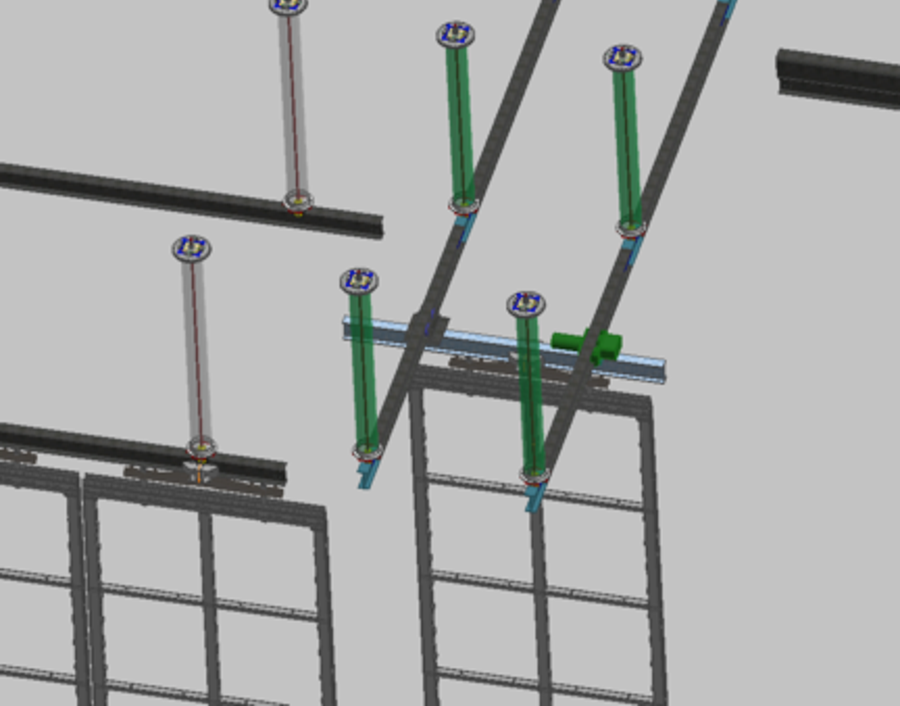
\includegraphics[width=\textwidth]{far-detector-single-phase/figures/Shuttle-1.pdf}
\end{minipage}
\begin{minipage}[c]{0.42\textwidth}
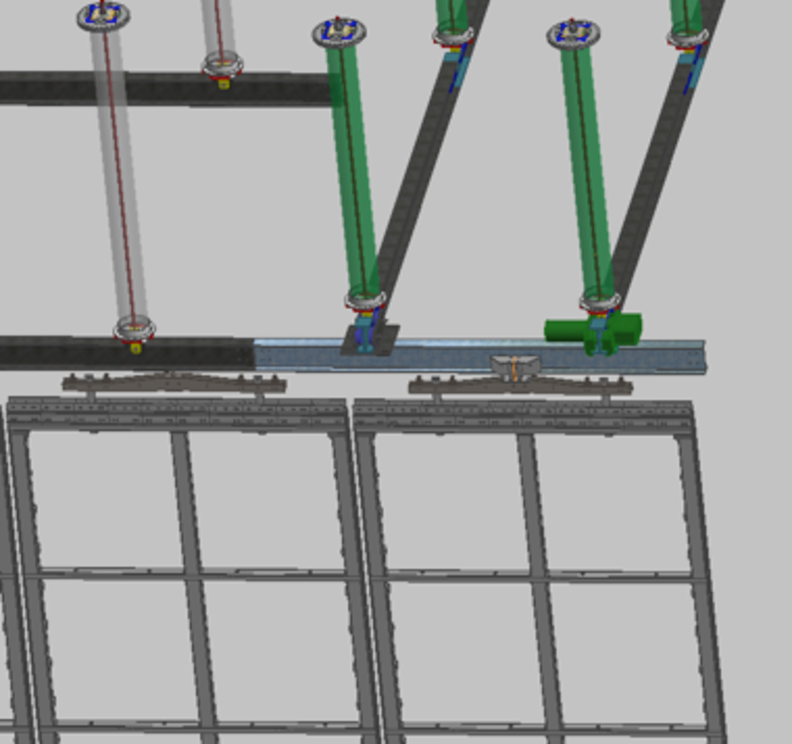
\includegraphics[width=\textwidth]{far-detector-single-phase/figures/shuttle-2.pdf}
\end{minipage}
\caption{3-D models of the shuttle beam end of the DSS. The figures show how an APA is translated into position using he North-South beams until it lines up with the correct row of I-beams.}
\label{shuttle}
\end{center}
\end{figure}

The DSS installation begins with the placement and alignment of all
the feedthroughs onto the flanges that are mounted to the warm vessel.
There are 25 feedthroughs per row and five rows for a total of 125
feedthroughs.  A fixture with a tooling ball will be attached to the
clevis of each feedthrough.  The $XY$ position in the horizontal plane
and the vertical $Z$ position of this tooling ball will be defined.  A
survey will be performed to determine the location of each tooling
ball center and $XY$ and $Z$ adjustments will be made to get the tooling
ball centers to within $\pm$3~mm.  The 6.4~m long I-beams will then be
raised and pinned to the clevis.  Each beam weights roughly 350~lbs.
A lifting tripod will be placed over each of the feedthroughs
supporting a beam and a $1/4 ^{''}$ cable will be fed through the top
flange of the feedthrough down the 14~m to the cryostat floor where it
will be attached to the I-beam.  The winches on each tripod will raise
the beam in unison in order to get it to the correct height to be
pinned to the feedthrough clevis.  Once the beams are mounted a final
survey of the beams will occur to ensure they are located and aligned
to each other properly.

A mock up of the shuttle system will be constructed to test the
mechanical interlock and drive systems for the shuttle beam
for each detector.  Tests will be conducted to evaluate the level of
misalignment between beams that can be tolerated and the amount of
positional control that can be achieved with the motorized trolley. It
is expected this will be finished prior to the TDR. At the time of the
TDR a larger prototype installation at Ash River will be under
construction. This prototype will use full scale elements and will be
used to develop the installation procedures and to also test the
detector installation process.

\fixme{concluding paragraph?}
